%% FEUP THESIS STYLE for LaTeX2e
%% how to use feupteses for MIEIC dissertations
%%
%% FEUP, JCL & JCF,  Wed Oct  4 16:32:24 2017
%%
%% PLEASE send improvements to jlopes at fe.up.pt and to jcf at fe.up.pt
%%

%%========================================
%% Commands: pdflatex pdis
%%           bibtex pdis
%%           makeindex pdis (only if creating an index) 
%%           pdflatex pdis
%% Alternative:
%%          latexmk -pdf pdis.tex
%%========================================

\documentclass[11pt,a4paper,twoside,openright]{report}
\usepackage[utf8]{inputenc}
%\usepackage[latin1]{inputenc}

%%%%%%% English version 

%% MIEIC options
\usepackage[mieic]{feupteses}                  % work version
%\usepackage[mieic,juri]{feupteses}             % juri verrion
%\usepackage[mieic,final]{feupteses}            % final version

%% Additional options for feupteses.sty: 
%% - portugues: titles, etc in portuguese
%% - onpaper: links are not shown (for paper versions)
%% - backrefs: include back references from bibliography to citation place

%%%%%%% Portuguese version

%\usepackage[mieic,portugues]{feupteses}        % work version
%\usepackage[mieic,portugues,juri]{feupteses}   % juri version
%\\usepackage[mieic,portugues,final]{feupteses}  % final version

%% Uncomment the next lines if side by side graphics used
%\usepackage[lofdepth,lotdepth]{subfig}
%\usepackage{graphicx}
%\usepackage{float}

%% Include color package
\usepackage{color}
\definecolor{cloudwhite}{cmyk}{0,0,0,0.025}

%% Include source-code listings package
\usepackage{listings}
\lstset{ %
 language=C,                        % choose the language of the code
 basicstyle=\footnotesize\ttfamily,
 keywordstyle=\bfseries,
 numbers=left,                      % where to put the line-numbers
 numberstyle=\scriptsize\texttt,    % the size of the fonts that are used for the line-numbers
 stepnumber=1,                      % the step between two line-numbers. If it's 1 each line will be numbered
 numbersep=8pt,                     % how far the line-numbers are from the code
 frame=tb,
 float=htb,
 aboveskip=8mm,
 belowskip=4mm,
 backgroundcolor=\color{cloudwhite},
 showspaces=false,                  % show spaces adding particular underscores
 showstringspaces=false,            % underline spaces within strings
 showtabs=false,                    % show tabs within strings adding particular underscores
 tabsize=2,	                    % sets default tabsize to 2 spaces
 captionpos=b,                      % sets the caption-position to bottom
 breaklines=true,                   % sets automatic line breaking
 breakatwhitespace=false,           % sets if automatic breaks should only happen at whitespace
 escapeinside={\%*}{*)},            % if you want to add a comment within your code
 morekeywords={*,var,template,new}  % if you want to add more keywords to the set
}

%% Uncomment to create an index (at the end of the document)
%\makeindex

%% Path to the figures directory
%% TIP: use folder ``figures'' to keep all your figures
\graphicspath{{figures/}}

%%----------------------------------------
%% TIP: if you want to define more macros, use an external file to keep them
%some macro definitions

% format
\newcommand{\class}[1]{{\normalfont\slshape #1\/}}

% entities
\newcommand{\Feup}{Faculdade de Engenharia da Universidade do Porto}

\newcommand{\svg}{\class{SVG}}
\newcommand{\scada}{\class{SCADA}}
\newcommand{\scadadms}{\class{SCADA/DMS}}

%%----------------------------------------

%%========================================
%% Start of document
%%========================================
\begin{document}

%%----------------------------------------
%% Information about the work
%%----------------------------------------
\title{Title of the Dissertation}
\author{Ângelo Miguel Tenreiro Teixeira}

%% Uncomment next line for date of submission
%\pdisdate{July 31, 2008}

%%Uncomment next line for copyright text if used
%\copyrightnotice{Name of the Author, 2008}

\supervisor{Supervisor}{Prof. João Correia Lopes}

%% Uncomment next line if necessary
%\supervisor{Second Supervisor}{Name of the Supervisor}

%% Uncomment committee stuff in the final version 
%\committeetext{Approved in oral examination by the committee:}
%\committeemember{Chair}{Doctor Name of the President}
%\committeemember{External Examiner}{Doctor Name of the Examiner}
%\committeemember{Supervisor}{Doctor Name of the Supervisor}

%\committeetext{Aprovado em provas públicas pelo Júri:}
%\committeemember{Presidente}{Nome do presidente do júri}
%\committeemember{Arguente}{Nome do arguente do júri}
%\committeemember{Vogal}{Nome do vogal do júri}

%% Uncomment signature line in the final on paper version
%\signature

%% Specify cover logo (in folder ``figures'')
\logo{uporto-feup.pdf}

%% Uncomment next line for additional text below the author's name (front page)
\additionalfronttext{Preparação da Dissertação}

%%----------------------------------------
%% Preliminary materials
%%----------------------------------------

% remove unnecssary \include{} commands
\begin{Prolog}
  \chapter*{Abstract}

Lorem ipsum dolor sit amet, consectetuer adipiscing elit. Sed vehicula
lorem commodo dui. Fusce mollis feugiat elit. Cum sociis natoque
penatibus et magnis dis parturient montes, nascetur ridiculus
mus. Donec eu quam. Aenean consectetuer odio quis nisi. Fusce molestie
metus sed neque. Praesent nulla. Donec quis urna. Pellentesque
hendrerit vulputate nunc. Donec id eros et leo ullamcorper
placerat. Curabitur aliquam tellus et diam. 

Ut tortor. Morbi eget elit. Maecenas nec risus. Sed ultricies. Sed
scelerisque libero faucibus sem. Nullam molestie leo quis
tellus. Donec ipsum. Nulla lobortis purus pharetra turpis. Nulla
laoreet, arcu nec hendrerit vulputate, tortor elit eleifend turpis, et
aliquam leo metus in dolor. Praesent sed nulla. Mauris ac augue. Cras
ac orci. Etiam sed urna eget nulla sodales venenatis. Donec faucibus
ante eget dui. Nam magna. Suspendisse sollicitudin est et mi. 

Fusce sed ipsum vel velit imperdiet dictum. Sed nisi purus, dapibus
ut, iaculis ac, placerat id, purus. Integer aliquet elementum
libero. Phasellus facilisis leo eget elit. Nullam nisi magna, ornare
at, aliquet et, porta id, odio. Sed volutpat tellus consectetuer
ligula. Phasellus turpis augue, malesuada et, placerat fringilla,
ornare nec, eros. Class aptent taciti sociosqu ad litora torquent per
conubia nostra, per inceptos himenaeos. Vivamus ornare quam nec sem
mattis vulputate. Nullam porta, diam nec porta mollis, orci leo
condimentum sapien, quis venenatis mi dolor a metus. Nullam
mollis. Aenean metus massa, pellentesque sit amet, sagittis eget,
tincidunt in, arcu. Vestibulum porta laoreet tortor. Nullam mollis
elit nec justo. In nulla ligula, pellentesque sit amet, consequat sed,
faucibus id, velit. Fusce purus. Quisque sagittis urna at quam. Ut eu
lacus. Maecenas tortor nibh, ultricies nec, vestibulum varius, egestas
id, sapien. 

Phasellus ullamcorper justo id risus. Nunc in leo. Mauris auctor
lectus vitae est lacinia egestas. Nulla faucibus erat sit amet lectus
varius semper. Praesent ultrices vehicula orci. Nam at metus. Aenean
eget lorem nec purus feugiat molestie. Phasellus fringilla nulla ac
risus. Aliquam elementum aliquam velit. Aenean nunc odio, lobortis id,
dictum et, rutrum ac, ipsum. 

Ut tortor. Morbi eget elit. Maecenas nec risus. Sed ultricies. Sed
scelerisque libero faucibus sem. Nullam molestie leo quis
tellus. Donec ipsum. Nulla lobortis purus pharetra turpis. Nulla
laoreet, arcu nec hendrerit vulputate, tortor elit eleifend turpis, et
aliquam leo metus in dolor. Praesent sed nulla. Mauris ac augue. Cras
ac orci. Etiam sed urna eget nulla sodales venenatis. Donec faucibus
ante eget dui. Nam magna. Suspendisse sollicitudin est et mi. 

Phasellus ullamcorper justo id risus. Nunc in leo. Mauris auctor
lectus vitae est lacinia egestas. Nulla faucibus erat sit amet lectus
varius semper. Praesent ultrices vehicula orci. 

Ut tortor. Morbi eget elit. Maecenas nec risus. Sed ultricies. Sed
scelerisque libero faucibus sem. Nullam molestie leo quis
tellus. Donec ipsum. 

\vspace*{10mm}\noindent
\textbf{Keywords}: keyword1, Keyword2, keyword3

\chapter*{Resumo}

Lorem ipsum dolor sit amet, consectetuer adipiscing elit. Sed vehicula
lorem commodo dui. Fusce mollis feugiat elit. Cum sociis natoque
penatibus et magnis dis parturient montes, nascetur ridiculus
mus. Donec eu quam. Aenean consectetuer odio quis nisi. Fusce molestie
metus sed neque. Praesent nulla. Donec quis urna. Pellentesque
hendrerit vulputate nunc. Donec id eros et leo ullamcorper
placerat. Curabitur aliquam tellus et diam. 

Ut tortor. Morbi eget elit. Maecenas nec risus. Sed ultricies. Sed
scelerisque libero faucibus sem. Nullam molestie leo quis
tellus. Donec ipsum. Nulla lobortis purus pharetra turpis. Nulla
laoreet, arcu nec hendrerit vulputate, tortor elit eleifend turpis, et
aliquam leo metus in dolor. Praesent sed nulla. Mauris ac augue. Cras
ac orci. Etiam sed urna eget nulla sodales venenatis. Donec faucibus
ante eget dui. Nam magna. Suspendisse sollicitudin est et mi. 

Fusce sed ipsum vel velit imperdiet dictum. Sed nisi purus, dapibus
ut, iaculis ac, placerat id, purus. Integer aliquet elementum
libero. Phasellus facilisis leo eget elit. Nullam nisi magna, ornare
at, aliquet et, porta id, odio. Sed volutpat tellus consectetuer
ligula. Phasellus turpis augue, malesuada et, placerat fringilla,
ornare nec, eros. Class aptent taciti sociosqu ad litora torquent per
conubia nostra, per inceptos himenaeos. Vivamus ornare quam nec sem
mattis vulputate. Nullam porta, diam nec porta mollis, orci leo
condimentum sapien, quis venenatis mi dolor a metus. Nullam
mollis. Aenean metus massa, pellentesque sit amet, sagittis eget,
tincidunt in, arcu. Vestibulum porta laoreet tortor. Nullam mollis
elit nec justo. In nulla ligula, pellentesque sit amet, consequat sed,
faucibus id, velit. Fusce purus. Quisque sagittis urna at quam. Ut eu
lacus. Maecenas tortor nibh, ultricies nec, vestibulum varius, egestas
id, sapien. 

Phasellus ullamcorper justo id risus. Nunc in leo. Mauris auctor
lectus vitae est lacinia egestas. Nulla faucibus erat sit amet lectus
varius semper. Praesent ultrices vehicula orci. Nam at metus. Aenean
eget lorem nec purus feugiat molestie. Phasellus fringilla nulla ac
risus. Aliquam elementum aliquam velit. Aenean nunc odio, lobortis id,
dictum et, rutrum ac, ipsum. 

Ut tortor. Morbi eget elit. Maecenas nec risus. Sed ultricies. Sed
scelerisque libero faucibus sem. Nullam molestie leo quis
tellus. Donec ipsum. Nulla lobortis purus pharetra turpis. Nulla
laoreet, arcu nec hendrerit vulputate, tortor elit eleifend turpis, et
aliquam leo metus in dolor. Praesent sed nulla. Mauris ac augue. Cras
ac orci. Etiam sed urna eget nulla sodales venenatis. Donec faucibus
ante eget dui. Nam magna. Suspendisse sollicitudin est et mi. 

Phasellus ullamcorper justo id risus. Nunc in leo. Mauris auctor
lectus vitae est lacinia egestas. Nulla faucibus erat sit amet lectus
varius semper. Praesent ultrices vehicula orci. 

Ut tortor. Morbi eget elit. Maecenas nec risus. Sed ultricies. Sed
scelerisque libero faucibus sem. Nullam molestie leo quis
tellus. Donec ipsum. 

\vspace*{10mm}\noindent
\textbf{Keywords}: keyword1, Keyword2, keyword3
  % the abstract
  \chapter*{Acknowledgments}

First, I would like to express my appreciation towards my supervisor Prof.\ João Correia Lopes for guiding me throughout this journey, correcting my wrongs and helping me learn throughout the writing of this document. I would also like to thank Eng.\ Marco Sousa, Eng.\ Pedro Dias and Eng.\ Vasco Ribeiro from the ZeroZero team, who allowed me to contribute to this project, learn about their challenges and contribute to them along the way. 

I would also like to thank my parents, who led me by example and shaped the basis of what I am today, and my sister, whom I am supposed to lead by example --- and hopefully in some years will be producing a document just like this of her own. I'd also like to give an \say{honorable mention} to my grandmother who naively thinks I am becoming a Doctor after completing this Masters' Thesis, which in itself gives a special kind of encouragement. Moreover, I would like to extend my gratitude towards my friends, many of which have crossed this bridge with me, providing support and many good memories. 

Finally, a message of appreciation to everyone that allowed me to extend my knowledge and shape my character to what it is today.

\vspace{10mm}
\flushleft{Ângelo Teixeira}
   % the acknowledgments
  \cleardoublepage
\thispagestyle{plain}

\vspace*{8cm}

\begin{flushright}
  \textsl{``Ceci n'est pas une citation.''}\\
\vspace*{1.5cm}
    Ângelo Teixeira
\end{flushright}
     % initial quotation if desired
  \cleardoublepage
  \pdfbookmark[0]{Table of Contents}{contents}
  \tableofcontents
  \cleardoublepage
  \pdfbookmark[0]{List of Figures}{figures}
  \listoffigures
  \cleardoublepage
  \pdfbookmark[0]{List of Tables}{tables}
  \listoftables
  \chapter*{Abbreviations}
\chaptermark{ABBREVIATIONS}
%\chapter*{Acrónimos}
%\chaptermark{ACRONIMOS}


\begin{flushleft}
\begin{tabular}{l p{0.8\linewidth}}
API      & Application Programming Interface\\
CRDT     & Conflict-free Replicated Data Type\\
CRUD     & Create, Read, Update, Delete\\
CSS      & Cascading Style Sheets\\
CmRDT    & Commutative Replicated Data Type\\
CvRDT    & Convergent Replicated Data Type\\
DNS      & Domain Name System\\
HTML     & Hypertext Markup Language\\
HTTP     & Hypertext Transfer Protocol\\
JS       & JavaScript\\
MO       & Multi-version Operations\\
NMO      & Non-Multi-version Operations\\
OT       & Operational Transformation\\
PPR      & Personalized PageRank \\
REST     & Representational State Transfer\\
TCP      & Transmission Control Protocol\\
UI       & User Interface\\
UX       & User Experience\\
\end{tabular}
\end{flushleft}

  % the list of abbreviations used
\end{Prolog}

%%----------------------------------------
%% Body
%%----------------------------------------
\StartBody

%% TIP: use a separate file for each chapter
\chapter{Introduction} \label{chap:intro}

\section*{}

As of today, millions of users follow their teams' games online to keep up-to-date regarding the events of a match \cite{kn:facebook-livestream-stats}. Some of those had a special connection to their hometown team, but since they play in way lower leagues and without much exposure, oftentimes the users end up missing information and losing the passion they once had for the hometown team.

There is a specific group of users, however, that keeps following the games of the smaller teams, and most importantly: sharing updates about them. One platform that allows users to do that, as of today, is zerozero.pt, from ZOS. This enables the most passionate fans that still watch the smaller leagues to share what is going on in the game, reporting the events and building the game's history, totally community-driven. This tool exists and is somewhat outdated, hence the opportunity to build something better.

The goal is to allow multiple users to report the events that happen in a sporting event, which show up for everyone following that match in real-time. As internet connectivity is often poor inside stadiums, the tool must allow offline work, which is synced whenever possible. This can generate many data inconsistencies, which must be handled by the tool.

In the past, work was already done trying to develop such a tool. This project will provide a fresh approach to this problem and the following sections provide more details on the key-objectives of the project. In Chapter \ref{chap:sota}, a comparison between the two projects is present, as well as a \textit{State of the Art} exploration on the multiple scopes of this project.

\section{Offline Availability} \label{sec:offline-avail-intro}

As previously stated, internet connection in stadiums is poor most of the time. Thus, the users must have the option to interact with the application and synchronize once possible. This will obviously lead to data consistency issues (i.e. two users report a goal, changing the result to "1-0" for example, but one of them is offline, so when it finally synchronizes, the result is already "3-2" and it should not overwrite it.)

More information on this and a proposed solution will be stated in Chapter \ref{sec:offline-avail}.

\section{Conflict Resolution} \label{sec:conflict-res-intro}

Another objective of the tool is to provide users with automatic conflict resolution when possible. Some strategies are depicted in the State of the Art section, in Chapter \ref{sec:conflict-res-sota}. Here, it is important to preserve the truth and the most up-to-date versions of data. In this scenario, there might not be a source of truth present to verify and validate all inputs, so other strategies must be used, such as an agreement-based implicit voting - if nobody questions a user's input, it must be true until stated otherwise.

Additionally, different strategies can be used to solve conflicts automatically, thus improving the user experience. More on the proposed solution can be found in Chapter \ref{sec:conflict-res} 

\section{Reputation System} \label{sec:rep-sys-intro}

The third key-objective of the application will be the reputation system. Currently, there already exists a ranking concept, as well as a "trusted" user, which is the equivalent to the maximum reputation and should be considered as the source of truth in case of conflict.

But what about the cases where two "non-trusted" users' inputs conflict, or even the case of two "trusted" users? Who should win? To resolve conflicts, an answer to these \textit{conundrums} is fundamental. Ergo a new reputation system is required, and more details are available in Chapter \ref{sec:rep-sys}.

\section{Summary} \label{sec:summary-intro}

Lorem ipsum dolor sit amet, consectetur adipiscing elit.
Mauris sem risus tempus a elit Chapter~\ref{chap:sota}.
Proin in mauris varius, auctor eros eu, accumsan est.
Suspendisse molestie elit in lacinia iaculis Chapter~\ref{chap:chap3}.
Sed lobortis sem non metus pharetra efficitur. Mauris tortor arcu,
pulvinar sit, molestie vitae libero Chapter~\ref{chap:chap4}.
In odio felis, consectetur vel rhoncus et, iaculis et nisi.
Suspendisse rutrum felis magna Chapter~\ref{chap:concl}.
 
\chapter{Background and Literature Review} \label{chap:sota}

\section*{}

This section will dive deep on previously done work related to this project. Since this is a complete application, there will be a comparison between similar existing applications. Then, there will be an analysis on the specific problems, and how they have been solved in the literature.

\section{Similar platforms}
On a basic level, this is a sporting-event following app. A similar platform would be 365scores.com \cite{kn:365scores-about}, which offers the following of the same events in real-time, however it does not offer the community-input feature of this proposed work.

Another platform that enables live viewing of sporting events is mycujoo.tv \cite{kn:mycujoo-about}. This one enables the teams themselves to livestream the game with video, and mark specific events as they happen, so that the viewers can revisit those moments in the video. It too lacks the community input feature when inserting the events; it is more geared towards the clubs sharing ability, rather than the fans'. 

This leaves zerozero.live as a singular app that will allow fans to contribute with the games' events in real-time, increasing engagement, which can be complemented with the enormous football-related database which can provide real-time statistics about the game.




\section{Offline Availability}\label{sec:offline-avail-sota}

\section{Conflict resolution}\label{sec:conflict-res-sota}

TODO Creative conflict resolution in realtime collaborative editing systems
TODO A Consensus-Driven Group Recommender System

\section{Reputation System}\label{sec:rep-sys-sota}

There are multiple examples of how reputation can be used in multi-user systems and how it can affect the group dynamics. Many refer refer to it as a solution to "Group Recommendations", which are based in \textbf{trust} among participants whereas others mention its ability to induce cooperation. Haveliwala, Taher TODO -> cite{Topic-sensitive PageRank} shows how the PageRank algorithm can be personalized so that each link among nodes has a different weight, in order to express a dynamic preference among nodes. Andersen et al. TODO->cite{Trust-based recommendation systems: An axiomatic approach} demonstrates multiple trust-based recommendation systems and how they comply with a set of relevant axioms. Most importantly, it shows how the aforementioned personalized PageRank (PPR) algorithm can be used to simulate a trust network among peers, by linking users with differently weighted connections. The greater the weight, the more a user trusts another, and the most likely it is for the Random Walk algorithm to choose that "path of trust". The latter also shows that PPR satisfies three out of five relevant axioms: \textbf{Symmetry}, \textbf{Positive Response}, \textbf{Transitivity}, but not Independence of Irrelevant Stuff and \textbf{Neighborhood Consensus}.
\begin{itemize}
    \item \textbf{Symmetry.} Isomorphic graphs result in corresponding isomorphic recommendations (anonymity), and the system is also symmetric
    \item \textbf{Positive response.} If a node’s recommendation is 0 and an edge is added to a + voter, then the former’s recommendation becomes +.
    \item \textbf{Transitivity.} For any graph (N, E) and disjoint sets $ A, B, C \subseteq N $ , for any source s, if s trusts A more than B, and s trusts B more than C, then s trusts A more than C.
    \item \textbf{Independence of Irrelevant Stuff (IIS).} A node’s recommendation is independent of agents not reach- able from that node. Recommendations are also independent of edges leaving voters.
    \item \textbf{Neighborhood consensus.} If a nonvoter’s neighbors unanimously vote +, then the recommendation of other nodes will remain unchanged if that node instead becomes a + voter.
\end{itemize}

Dellarocas, Chrysanthos TODO-> cite {Reputation Mechanisms} shows examples of how multiple platforms handle their user reputations mechanisms. It also states prevention of moral hazard as an objective of reputation systems, as they can deter moral hazard by acting as santioning devices. If the community punishes users with a history of bad behavior and if the punishment exceeds the gains from "cheating", then the threat of public revelation of a user's cheating behavior is an incentive for users to cooperate instead. It further elaborates on the reputation dynamics of a multi-user application: 
\begin{itemize}
    \item \textbf{Initial Phase} - In most cases, reputation effects begin to work immediately and in fact are strongest during the initial phase, when users must work hard to establish a reputation. A case where reputation effects may fail to work is when short-run users are “too cautious” when compared to the long-run ones and therefore update their beliefs too slowly in order for the long-run user to find it profitable to try to build a reputation.
    \item \textbf{Steady state} (or lack thereof) - In their simplest form, reputation games are characterized by an equilibrium in which the long-run player repeatedly plays the safe action, also known as the Stackelberg action, with high probability and the player’s reputation converges to the Stackelberg type (always collaborating and no cheating).
\end{itemize}

These dynamics have important repercussions for reputation systems. Dellarocas goes on to say that if the entire feedback history of a seller is made available to users and if a colaborator stays on the system long enough, once he establishes an initial reputation for honesty will be tempted to cheat buyers every now and then. In the long term, this behavior will lead to an eventual collapse of his reputation and therefore of cooperative behavior.

Bakos and  Dellarocas TODO->cite{Cooperation Without Enforcement? A comparative analysis of litigation and online reputation as quality assurance mechanisms} presents a model for a reputation system and explores the ability of online reputation mechanisms to efficiently induce cooperation, compared to contractual arrangements relying on the threat of litigation. It concludes that the effectiveness of a reputation mechanism in inducing cooperative behavior has a discontinuous relationship to the frequency of transactions that are affected by this mechanism: A certain degree of participation is required before reputation can induce a significant level of cooperation. Once this threshold is reached, however, the power of reputation springs to life in a discontinuous fashion and high levels of cooperation can be supported.

Dellarocas TODO-> cite{How often should reputation mechanisms update a trader's reputation profile?} concludes that reputation mechanisms can induce higher cooperation and efficiency if, instead of publishing new ratings as soon as they are received, they only update a user's public reputation profile every k transactions with a summary statistic of a user's last ratings. In settings with noise, infrequent updating increases efficiency because it decreases the adverse consequence of spurious negative ratings. At the same time, however, infrequent updating increases a user's short-term profits from cheating and thus the minimum future punishment threat that can sustain cooperation.

In TODO->cite {User’s understanding of reputation issues in a community based mobile app}, tests were made in order to understand the reputation issues for users. These were made in Waze, a GPS-like driving assistant with crowd collaboration for road events. Even though this and zerozero.live are somewhat different, some paralelisms can be made and some gathered information still applies. They concluded that it was hard for users to recognize where the information came from, and if it was reliable at all. Furthermore, users did not care much about their reputation when submitting information (i.e. if they heard about some road event, they would publish it without verifying it), maybe this is somewhat different from our use-case of sporting events, as users are either actually watching the game, or following it from a reliable source. Additionally, when users knew the source of data, they tended to trust people in their close circle (e.g. familly and friends) and the main conclusion is that the app needed to better convey the reputation of the source to let the consumers know how much they can or should trust the source.

Resnick et al. TODO->cite{Reputation Systems} elaborate about reputation systems and their generic importance on the web. It is more geared towards e-commerce examples where people investigate the reputation before interacting with each other. It mentions three important properties reputation systems should have:
\begin{itemize}
    \item Long-lived entities that inspire an expectation of future interaction. If the entities are short-lived, their reputation matters little;
    \item Capture and distribution of feedback about current interactions (such information must be visible in the future);
    \item Use of feedback to guide trust decisions;
\end{itemize}
In the zerozero.live case, it might be hard to get expressive feedback from users regarding other users. Therefore it is important to have some kind of implicit voting in place. Additionally, users are more inclined to express feedback when they disagree than when they agree, which means that the lack of negative feedback must be considered as some sort of positive feedback in order to balance the system. Besides, users won't see the reputation of other users beforehand in order to decide to interact or not, as they simply enter the event without knowing who is also there, so it is important that they can see the reputation, or a variant of it (i.e. some relative reputation based on the current group of users) while they are at the event (e.g. Showing it next to the user's name).

Melnikov A, Lee J Rivera V et al. TODO cite{Towards dynamic interaction-based reputation models} presents a dynamic interaction based reputation model (DIB-RM), which is further evaluated in TODO cite {Expressing Trust with Temporal Frequency of User Interaction in Online Communities}. It presents a method to measure reputation as a function of user interaction frequency, also contemplating a reputation decay if the users stop contributing to the platform. 

The aforementioned method is also present in TODO-> cite{Harnessing wisdom of the crowds dynamics for time-dependent reputation and ranking}, where the authors present a way to harness the "wisdom of the crowds", very much in line with what is required in zerozero.live, since there is no express authority during the event. It presents an example of a document sharing system and the approach to rank the documents based on the amount of readers, the reputation of the author, the time dynamics of reader consumption, and the time dynamics of documents contributed by the user. This last one manifests indirectly, but is still relevant: it means that if a user has less frequent readers on their documents, their reputation will decrease, so the contribution to the main document's reputation - the one they are reading now - will be smaller.
Reputation values scale between 0 and 1 and it sticks to the following rules:
\begin{enumerate}
    \item Every time a user consumes a document from an author, the author gains reputation according to:
    \[newRep = oldRep + (1 - oldRep) * repReward\]
    $repReward$ is a constant between 0 and 1 and should consider the number of entities in the system. As the paper states: "If the number of expected consumers is in the order of hundreds or thousands, then an overly high value of $repReward$ will potentially cause popular content to quickly converge towards 1 making it difficult to differentiate between similarly popular content.".
    \item Every time a user consumes a document, the document gains "reputation" - meaning popularity in this case - according to the same formula of (1):
    \[newRep = oldRep + (1 - oldRep) * repReward\]
    \item In order to take time dynamics into account, reputation should decrease over time, so that a "rich-get-richer" paradigm can be avoided. This is achieved by the following equation (both for users and for documents):
    \[newRep = oldRep * decayCoeff^k\]
    $decayCoeff$ represents how much the reputation will change, and $k$ is the amount of time units that have passed since the last reputation update, i.e for a time unit of "days", $k$ will be 0 in the first 24h, 1 in the next day, 7 in a week, and so on. This decouples the algorithm from the logistics, since the algorithm can now run in a fixed frequency, independently from the time units, and every time it re-calculates, it will give an accurate value. However, if for example the time unit is "day", and the algorithm updates every week only, there will be an offset of 6 days where the value will be outdated.
    \item Users with higher reputation matter more when calculating the document reputation changes:
    \[newRep = oldRep * repConsumer * B\]
    $B$ is a constant within [0, 1] representing to what extent the user reputation $repConsumer$ will influence the document's reputation.

    This system can be adapted and applied in zerozero.live if we map user inputs in an event as documents. However, we will be ranking users instead of "documents" - inputs - even though they will also have reputation values. This will be explained in more detail in (TODO section explaining rep algorithm according to this - revive the rule numbers there, since they will be referenced).
    
\end{enumerate} 
\chapter{Another Chapter}\label{chap:chap3}

\section*{}

Lorem ipsum dolor sit amet, consectetur adipiscing elit. Donec semper
finibus massa sed tristique. Nullam vel dui a nisl vulputate
placerat. Phasellus non mi ornare, ultrices lectus eget, cursus
ante. Sed sit amet euismod massa. Suspendisse ornare est dolor, at
egestas eros rutrum vel\footnote{Another footnote.}.

Aliquam nunc dui, sagittis eu molestie vitae, consectetur ut sem. Nam
nunc diam, bibendum a tellus ac, tincidunt sagittis orci. Aenean dolor
ex, convallis nec mi a, porttitor feugiat ante. Proin eu felis
libero. Curabitur efficitur eleifend augue et tincidunt. Aliquam erat
volutpat. Curabitur sit amet justo dui.

\section{A Section with an Equation}

In suscipit mauris a nunc. Pellentesque gravida. Morbi quam
lacus, pretium eget, tincidunt vulputate, interdum sed,
turpis. Curabitur quis est.

Duis tempor condimentum ante:
\begin{eqnarray}
CIF_1: \hspace*{5mm}F_0^j(a) &=& \frac{1}{2\pi \iota} \oint_{\gamma} \frac{F_0^j(z)}{z - a} dz\\
CIF_2: \hspace*{5mm}F_1^j(a) &=& \frac{1}{2\pi \iota} \oint_{\gamma} \frac{F_0^j(x)}{x - a} dx \label{eq:cif}
\end{eqnarray}

Equation~\ref{eq:cif} lorem ipsum dolor sit amet, consectetuer
adipiscing elit. Suspendisse tincidunt viverra elit. Donec tempus
vulputate mauris. Donec arcu. Vestibulum condimentum porta
justo. Curabitur ornare tincidunt lacus. Curabitur ac massa vel ante
tincidunt placerat. Cras vehicula semper elit. Curabitur gravida, est
a elementum suscipit, est eros ullamcorper quam, sed cursus velit
velit tempor neque. 

Phasellus imperdiet, orci vel pretium sollicitudin, magna nunc
ullamcorper augue, non venenatis dui nunc quis massa. Pellentesque
dolor elit, dapibus venenatis, viverra ultricies, accumsan cursus,
orci. Aliquam erat volutpat. Mauris ornare tristique leo. Maecenas
eros. Curabitur velit nunc, tincidunt vitae, dictum posuere, pulvinar
nec, diam. Sed lectus lorem, congue vel, dignissim
laoreet, blandit a, nisi. Aenean nunc ligula, tincidunt eu, hendrerit
vel, suscipit non, erat. Aliquam gravida. Integer non pede. In laoreet
augue id leo. Mauris placerat~\cite{kn:ZPMD97}: 

\begin{itemize}
\item \textbf{Componentes} --- Suspendisse auctor mattis augue \emph{push};
\item \textbf{Praesent} --- Sit amet sem maecenas eleifend facilisis leo;
\item \textbf{Pellentesque} --- Habitant morbi tristique senectus et netus.
\end{itemize}

\subsection{A Subsection with a Figure}

In est justo, tristique in Figure~\ref{fig:arch} %on page~\pageref{fig:arch}
iverra ultricies, accumsan cursus,

\begin{figure}[t]
  \begin{center}
    \leavevmode
    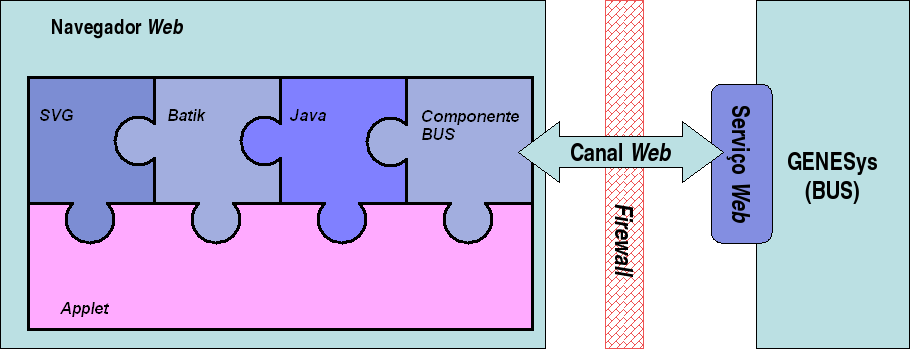
\includegraphics[width=0.86\textwidth]{puzzle}
    \caption{Proposed Architecture}
    \label{fig:arch}
  \end{center}
\end{figure}

Loren ipsum dolor sit amet, consectetuer adipiscing elit. 
Praesent sit amet sem. Maecenas eleifend facilisis leo. Vestibulum et
mi. Aliquam posuere, ante non tristique consectetuer, dui elit
scelerisque augue, eu vehicula nibh nisi ac est. Suspendisse elementum
sodales felis. Nullam laoreet fermentum urna. 

Pellentesque habitant morbi tristique senectus et netus et
malesuada fames ac turpis egestas. Fusce feugiat, elit ac placerat
fermentum, augue nisl ultricies eros, id fringilla enim sapien eu
felis. Vestibulum ante ipsum primis in faucibus orci luctus et
ultrices posuere cubilia Curae; Sed dolor mi, porttitor quis,
condimentum sed luctus. 

\subsection{Another subsection with  Tables}

Aenean rhoncus mauris sed ante tincidunt efficitur. Nam quis turpis
eleifend, rutrum nunc quis, interdum ipsum Table~\ref{tab:exemplo1}.
Suspendisse at sem nibh. Donec dapibus, lorem non faucibus dictum,
dolor sem porta mauris, id blandit nisl mi nec urna.
Suspendisse pretium diam massa Table~\ref{tab:exemplo2},
id tincidunt enim fringilla non. Ut posuere purus tortor, a dignissim
felis tempus gravida. Donec a facilisis nisi. Aliquam pulvinar lectus
sit amet libero fermentum, id blandit neque imperdiet. Phasellus
consequat blandit lacus ut bibendum. Integer eleifend condimentum
purus, vitae porttitor est. Ut vel ultrices nulla, quis volutpat quam.

\begin{table}[t]
  \centering
  \caption{A Simple Table}
\begin{tabular}{| l | l |}
	\hline
\textbf{Acronym} & \textbf{Description}\\
	\hline
	\hline
        ADT   & \emph{Abstract Data Type}\\\hline
        ANDF  & \emph{Architecture-Neutral Distribution Format}\\\hline
        API   & \emph{Application Programming Interface}\\
	\hline
\end{tabular}
  \label{tab:exemplo1}
\end{table}

Integer quis pede. Fusce nibh. Fusce nec erat vel mi condimentum
convallis. Sed at tortor non mauris pretium aliquet. In in lacus in
dolor molestie dapibus. Suspendisse potenti. Pellentesque sagittis
porta erat. Mauris sodales sapien id augue. Nam eu dolor. Donec sit
amet turpis non orci rhoncus commodo. Etiam condimentum commodo
libero.

Mauris pede. Curabitur faucibus dictum nibh. Proin tincidunt diam
vitae mauris. Sed hendrerit dolor vel ipsum. Nullam dapibus. Vivamus
tellus diam, egestas sit amet, vulputate non, vulputate id, eros. Nunc
sit amet nibh eget nibh imperdiet ornare. Cras vehicula mattis
ipsum. Sed diam arcu, semper at, gravida vitae, fermentum et,
nulla. Aenean massa orci, tristique nec, rutrum id, fringilla eget,
erat. Curabitur nulla ipsum, aliquam sed, rutrum vitae, semper quis,
ante. Fusce at nunc in dolor condimentum tempor. Duis sit amet massa. 

Curabitur convallis nulla quis risus. Nulla mollis porttitor
purus. Fusce ultricies odio at ligula pellentesque suscipit. Nulla
velit libero, blandit a, aliquet quis, hendrerit id, arcu. Phasellus
porttitor porttitor purus. Suspendisse velit tortor, fringilla sit
amet, commodo a, ultrices et, mi. Donec eu metus in erat ornare
adipiscing. Praesent varius mi ac nunc. Vestibulum leo lacus,
elementum in, vestibulum sit amet, hendrerit at, justo. Sed sit amet
neque. Donec libero risus, commodo sit amet, dignissim ut, tincidunt
a, eros. Ut non lacus quis tortor mattis ullamcorper. Vivamus
consequat augue vel erat. Sed tincidunt. Sed leo eros, ornare a,
pulvinar non, mattis quis, nibh. Aliquam faucibus mi ac nisi.

Pellentesque habitant morbi tristique senectus et netus et malesuada
fames ac turpis egestas. Duis aliquet, libero sit amet ornare viverra,
augue erat interdum dolor, vitae tincidunt lorem erat a lacus. Sed
lectus nisi, auctor in, hendrerit a, molestie vel, lectus. Cum sociis
natoque penatibus et magnis dis parturient montes, nascetur ridiculus
mus. Duis lacinia tempor dui. Vivamus rhoncus, tellus a viverra
dignissim, pede dui adipiscing odio, non faucibus metus mi gravida
eros. Nullam a tellus ut velit elementum tempus. Aenean rutrum
convallis tellus. Vestibulum nulla ante, dapibus ut, lobortis ut,
varius sed, nisl. Fusce lobortis. Sed ac lorem. Nulla tincidunt nulla
eget leo. Maecenas ac lectus eu neque ultrices pharetra. Curabitur a
risus nec arcu placerat tempor. Suspendisse magna nisl, viverra a,
adipiscing eget, ornare ultricies, ligula. Maecenas eu ligula vitae
eros convallis dignissim. 

\begin{table}[t]
  \centering
  \caption{A more Complex Table}
\begin{tabular}{|c|r@{.}lr@{.}lr@{.}l||r|}
	\hline
\multicolumn{8}{|c|}
	{\rule[-3mm]{0mm}{8mm}Iteration  $k$ of $f(x_n)$} \\
\textbf{\em k}
	& \multicolumn{2}{c}{$x_1^k$}
	& \multicolumn{2}{c}{$x_2^k$}
	& \multicolumn{2}{c||}{$x_3^k$}
	& comments \\ \hline \hline
0   & -0&3        & 0&6        &  0&7         & - \\
1   &  0&47102965 & 0&04883157 & -0&53345964  & $\delta<\epsilon$ \\
2   &  0&49988691 & 0&00228830 & -0&52246185  & $\delta < \varepsilon$ \\
3   &  0&49999976 & 0&00005380 & -0&523656    &   $N$ \\
4   &  0&5        & 0&00000307 & -0&52359743  & \\
\vdots	& \multicolumn{2}{c}{\vdots}
	& \multicolumn{2}{c}{$\ddots$}
	& \multicolumn{2}{c||}{\vdots}  & \\
7   &  0&5   & 0&0    & \textbf{-0}&\textbf{52359878}
		 & $\delta<10^{-8}$ \\ \hline
\end{tabular}
  \label{tab:exemplo2}
\end{table}

Loren ipsum dolor sit amet, consectetuer adipiscing elit. 
Praesent sit amet sem. Maecenas eleifend facilisis leo. Vestibulum et
mi. Aliquam posuere, ante non tristique consectetuer, dui elit
scelerisque augue, eu vehicula nibh nisi ac est. Suspendisse elementum
sodales felis. Nullam laoreet fermentum urna.  Cras vehicula mattis
ipsum. Sed diam arcu, semper at, gravida vitae, fermentum et,
nulla. Aenean massa orci, tristique nec, rutrum id, fringilla eget,
erat. Curabitur nulla ipsum, aliquam sed, rutrum vitae, semper quis,
ante. Fusce at nunc in dolor condimentum tempor

Duis eget diam. In est justo, tristique in, lacinia vel, feugiat eget,
quam. Pellentesque habitant morbi tristique senectus et netus et
malesuada fames ac turpis egestas. Fusce feugiat, elit ac placerat
fermentum, augue nisl ultricies eros, id fringilla enim sapien eu
felis. Vestibulum ante ipsum primis in faucibus orci luctus et
ultrices posuere cubilia Curae; Sed dolor mi, porttitor quis,
condimentum sed luctus. 

\section{Yet Another Section}

Loren ipsum dolor sit amet, consectetuer adipiscing elit. 
Praesent sit amet sem. Maecenas eleifend facilisis leo. Vestibulum et
mi. Aliquam posuere, ante non tristique consectetuer, dui elit
scelerisque augue, eu vehicula nibh nisi ac est. Suspendisse elementum
sodales felis. Nullam laoreet fermentum urna. 

Duis eget diam. In est justo, tristique in, lacinia vel, feugiat eget,
quam. Pellentesque habitant morbi tristique senectus et netus et
malesuada fames ac turpis egestas. Fusce feugiat, elit ac placerat
fermentum, augue nisl ultricies eros, id fringilla enim sapien eu
felis. Vestibulum ante ipsum primis in faucibus orci luctus et
ultrices posuere cubilia Curae; Sed dolor mi, porttitor quis,
condimentum sed luctus. 

\section{Summary}

Lorem ipsum dolor sit amet, consectetur adipiscing elit. Aliquam non
ultricies nibh, ut cursus neque. Vestibulum mattis ac odio ac
euismod. Integer posuere nibh odio, a fermentum massa iaculis
sed. 

Mauris eu mattis erat, eget feugiat quam. Fusce ut
justo sed lorem eleifend ornare ac vitae mi. Donec eu magna eget metus
porta vulputate. Aenean elementum turpis gravida elit iaculis
bibendum. 

% \include{chapter4}
\chapter{Conclusions and Future Work} \label{chap:concl}

\section*{}

Nullam eleifend condimentum nibh. Integer leo nibh, consequat eget,
mollis et, sagittis ac, felis. Duis viverra pede in pede. Phasellus
molestie placerat leo. Praesent at tellus a augue congue molestie.
Integer eu ante pellentesque, viverra orci vitae, facilisis
risus. Nunc eget pulvinar orci.

Proin sed justo eu sapien eleifend elementum. Pellentesque habitant
morbi tristique senectus et netus et malesuada fames ac turpis
egestas.  Praesent id lobortis magna, ut interdum enim.

\section{Results}

Lorem ipsum dolor sit amet, consectetuer adipiscing elit. Etiam non
felis sed odio rutrum ultrices. Donec tempor dolor. Vivamus justo
neque, tempus id, ullamcorper in, pharetra non, tellus. Praesent eu
orci eu dolor congue gravida. Sed eu est. Donec pulvinar, lectus et
eleifend volutpat, diam sapien sollicitudin arcu, a sagittis libero
neque et dolor. Nam ligula. Cras tincidunt lectus quis nunc. Cras
tincidunt congue turpis. Nulla pede velit, sagittis a, faucibus vitae,
porttitor nec, ante. Nulla ut arcu. Cras eu augue at ipsum feugiat
hendrerit. Proin sed justo eu sapien eleifend elementum. Pellentesque
habitant morbi tristique senectus et netus et malesuada fames ac
turpis egestas. Vivamus quam lacus, pharetra vel, aliquam vel,
volutpat sed, nisl. 

Nullam erat est, vehicula id, tempor non, scelerisque at,
tellus. Pellentesque tincidunt, ante vehicula bibendum adipiscing,
lorem augue tempor felis, in dictum massa justo sed metus. Suspendisse
placerat, mi eget molestie sodales, tortor ante interdum dui, ac
sagittis est pede et lacus. Duis sapien. Nam ornare turpis et
magna. Etiam adipiscing adipiscing ipsum. Fusce sodales nisl a
arcu. Cras massa leo, vehicula facilisis, commodo a, molestie
faucibus, metus. Suspendisse potenti. Duis sagittis. Donec porta. Sed
urna. Maecenas eros. Vivamus erat ligula, pharetra sit amet, bibendum
et, fermentum sed, dolor. 

\section{Further Work}

Lorem ipsum dolor sit amet, consectetuer adipiscing elit. Aliquam
tempor tristique risus. Suspendisse potenti. Fusce id eros. In eu
enim. Praesent commodo leo. Nullam augue. Pellentesque tellus. Integer
pulvinar purus a dui convallis consectetuer. In adipiscing, orci vitae
lacinia semper, sapien elit posuere sem, ac euismod ipsum elit tempus
urna. Aliquam erat volutpat. Nullam suscipit augue sed
felis. Phasellus faucibus accumsan est. 

Aliquam felis justo, facilisis sit amet, bibendum ut, tempus ac,
dolor. Sed malesuada. Nunc non massa. In erat. Nulla
facilisi. Phasellus blandit, est in accumsan cursus, libero augue
elementum leo, vitae auctor mauris nisl ac tortor. Cras porttitor
ornare elit. Fusce at lorem. Sed lectus tortor, vestibulum id, varius
a, condimentum nec, lectus. Maecenas in nisi et magna pretium
aliquam. Pellentesque justo elit, feugiat nec, tincidunt a, dignissim
vel, ipsum. Sed nunc. Vestibulum ante ipsum primis in faucibus orci
luctus et ultrices posuere cubilia Curae; Aliquam tempus rhoncus
leo. Donec neque quam, cursus sit amet, ultricies varius, semper non,
pede. Donec porttitor. Sed aliquet feugiat elit.  

\vspace*{12mm}

Lorem ipsum dolor sit amet, consectetuer adipiscing elit. Phasellus
tellus pede, auctor ut, tincidunt a, consectetuer in, felis. Mauris
quis dolor et neque accumsan pellentesque. Donec dui magna,
scelerisque mattis, sagittis nec, porta quis, nulla. Vivamus quis
nisl. Etiam vitae nisl in diam vehicula viverra. Sed sollicitudin
scelerisque est. Nunc dapibus. Sed urna. Nulla gravida. Praesent
faucibus, risus ac lobortis dignissim, est tortor laoreet mauris,
dictum pellentesque nunc orci tincidunt tellus. Nullam pulvinar, leo
sed vestibulum euismod, ante ligula elementum pede, sit amet dapibus
lacus tortor ac nisl. Morbi libero. Integer sed dolor ac lectus
commodo iaculis. Donec ut odio.  
 

%% comment next 2 commands if numbered appendices are not used
\appendix
\chapter{Services Architecture} \label{ap1:annex-high-level-arch}

This annex contains the architecture diagram of the implemented solution, representing all of its components, as explained in Chapter~\ref{chap:solution}.

\begin{landscape}
    \begin{figure}
       \centering
        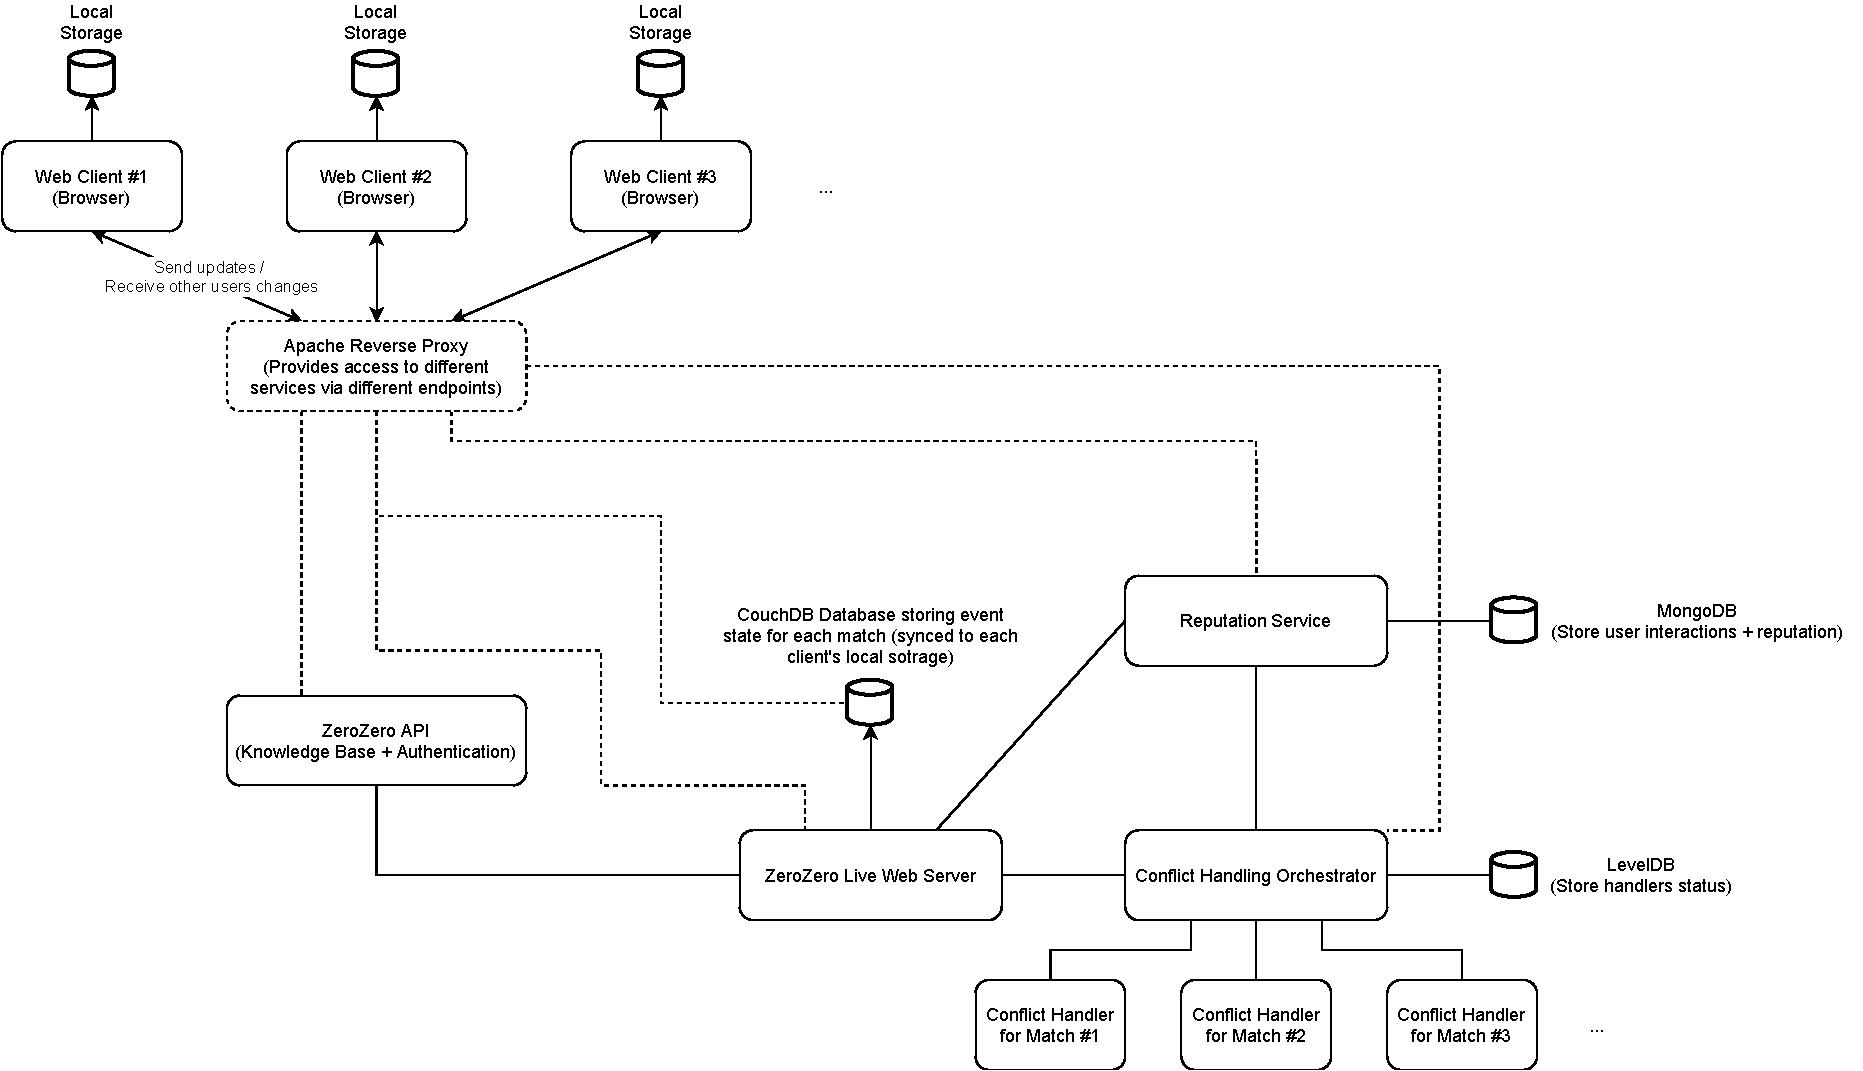
\includegraphics[height=0.9\textheight]{zerozerolive-arch.pdf}
        \caption{Services Architecture of the Application}
        \label{fig:annex-high-level-arch}
    \end{figure}
    \end{landscape}

\chapter{ZeroZero API events list} \label{annex:api-events}

\begin{longtable}{| p{.20\textwidth} | p{.60\textwidth} | p{.20\textwidth} |} 
    \caption{ZeroZero API events list (some fields were omitted for better reading purposes)} \\
    \hline
    \textbf{Event Id} & \textbf{Event Name} & \textbf{Category} \\ \hline
    \endfirsthead       
    \hline    
    \textbf{Event Id} & \textbf{Event Name} & \textbf{Category} \\ \hline       
    \endhead      
    8 & Estatísticas & 6 \\ \hline
    16 & Tempo Adicional & 6 \\ \hline
    24 & Info Jogador & 6 \\ \hline
    26 & Classificação & 6 \\ \hline
    29 & Outro Resultado & 6 \\ \hline
    43 & Lance polémico & 6 \\ \hline
    52 & VAR & 6 \\ \hline
    64 & Estatísticas Jogo & 6 \\ \hline
    78 & Fora de jogo & 6 \\ \hline
    79 & Castigado & 6 \\ \hline
    80 & Árbitros & 6 \\ \hline
    81 & Apresentação VAR & 6 \\ \hline
    83 & Canto & 6 \\ \hline
    3 & Comentário & 5 \\ \hline
    19 & Informação & 5 \\ \hline
    20 & Lesão grave & 5 \\ \hline
    22 & Homem do Jogo & 5 \\ \hline
    31 & Informação R. & 5 \\ \hline
    32 & Onzes Definidos & 5 \\ \hline
    36 & Info Pré-Jogo & 5 \\ \hline
    42 & Opinião & 5 \\ \hline
    46 & Antevisão & 5 \\ \hline
    47 & Rescaldo & 5 \\ \hline
    49 & Atualização de Resultado & 5 \\ \hline
    50 & Suplentes & 5 \\ \hline
    54 & Espetadores & 5 \\ \hline
    55 & Lesão & 5 \\ \hline
    5 & Substituição & 4 \\ \hline
    9 & Apito Inicial & 3 \\ \hline
    10 & Fim 1ª Parte & 3 \\ \hline
    11 & Início 2ª Parte & 3 \\ \hline
    12 & Fim 2ª Parte & 3 \\ \hline
    13 & Apito Final & 3 \\ \hline
    14 & Início Prolong. & 3 \\ \hline
    15 & Fim Prolong. & 3 \\ \hline
    56 & Fim 1ª Parte Prolongamento & 3 \\ \hline
    57 & Início 2ª Parte Prolongamento & 3 \\ \hline
    2 & Cartão Amarelo & 2 \\ \hline
    4 & Cartão Vermelho & 2 \\ \hline
    1 & Golo & 1 \\ \hline
    6 & Oportunidade Grande & 1 \\ \hline
    7 & Auto-Golo & 1 \\ \hline
    17 & Penalti Marcado & 1 \\ \hline
    18 & Penalti Falhado & 1 \\ \hline
    23 & Penalti Assin. & 1 \\ \hline
    35 & Penálti falhado & 1 \\ \hline
    44 & Golo invalidado & 1 \\ \hline
    53 & Oportunidade Pequena & 1 \\ \hline
    67 & Bola à barra & 1 \\ \hline
    68 & Bola ao poste & 1 \\ \hline
    84 & Assistência & 1 \\ \hline
    25 & Estatisticas 11 & 0 \\ \hline
    27 & Estatísticas Nac & 0 \\ \hline
    28 & Vídeo & 0 \\ \hline
    30 & Fotos & 0 \\ \hline
    34 & Penálti marcado & 0 \\ \hline
    37 & Info Pós-Jogo & 0 \\ \hline
    38 & JOG - Golos na Seleção (Único) & 0 \\ \hline
    39 & EQ - Resultados & 0 \\ \hline
    41 & Sondagem & 0 \\ \hline
    45 & Curiosidade PM & 0 \\ \hline
    48 & Fim de Relato & 0 \\ \hline
    51 & Bola ao ferro & 0 \\ \hline
    58 & Opinião com Foto & 0 \\ \hline
    60 & 5.ª falta & 0 \\ \hline
    61 & Time-out & 0 \\ \hline
    62 & Livre 10m assinalado & 0 \\ \hline
    63 & Cincos definidos & 0 \\ \hline
    65 & 5x4+GR & 0 \\ \hline
    66 & Faltas (Futsal) & 0 \\ \hline
    69 & Livre 10m Falhado & 0 \\ \hline
    70 & Livre 10m marcado & 0 \\ \hline
    71 & Livre direto assinalado & 0 \\ \hline 
    72 & Livre direto marcado & 0 \\ \hline
    73 & Livre direto falhado & 0 \\ \hline
    74 & 10.ª falta & 0 \\ \hline
    75 & 15.ª falta & 0 \\ \hline
    76 & 20.ª falta & 0 \\ \hline
    77 & Cartão Azul & 0 \\ \hline
    % \label{tab:myfirstlongtable}
\end{longtable}

% \begin{figure}[h]
%     \centering
%     \rotatebox{90}{
%         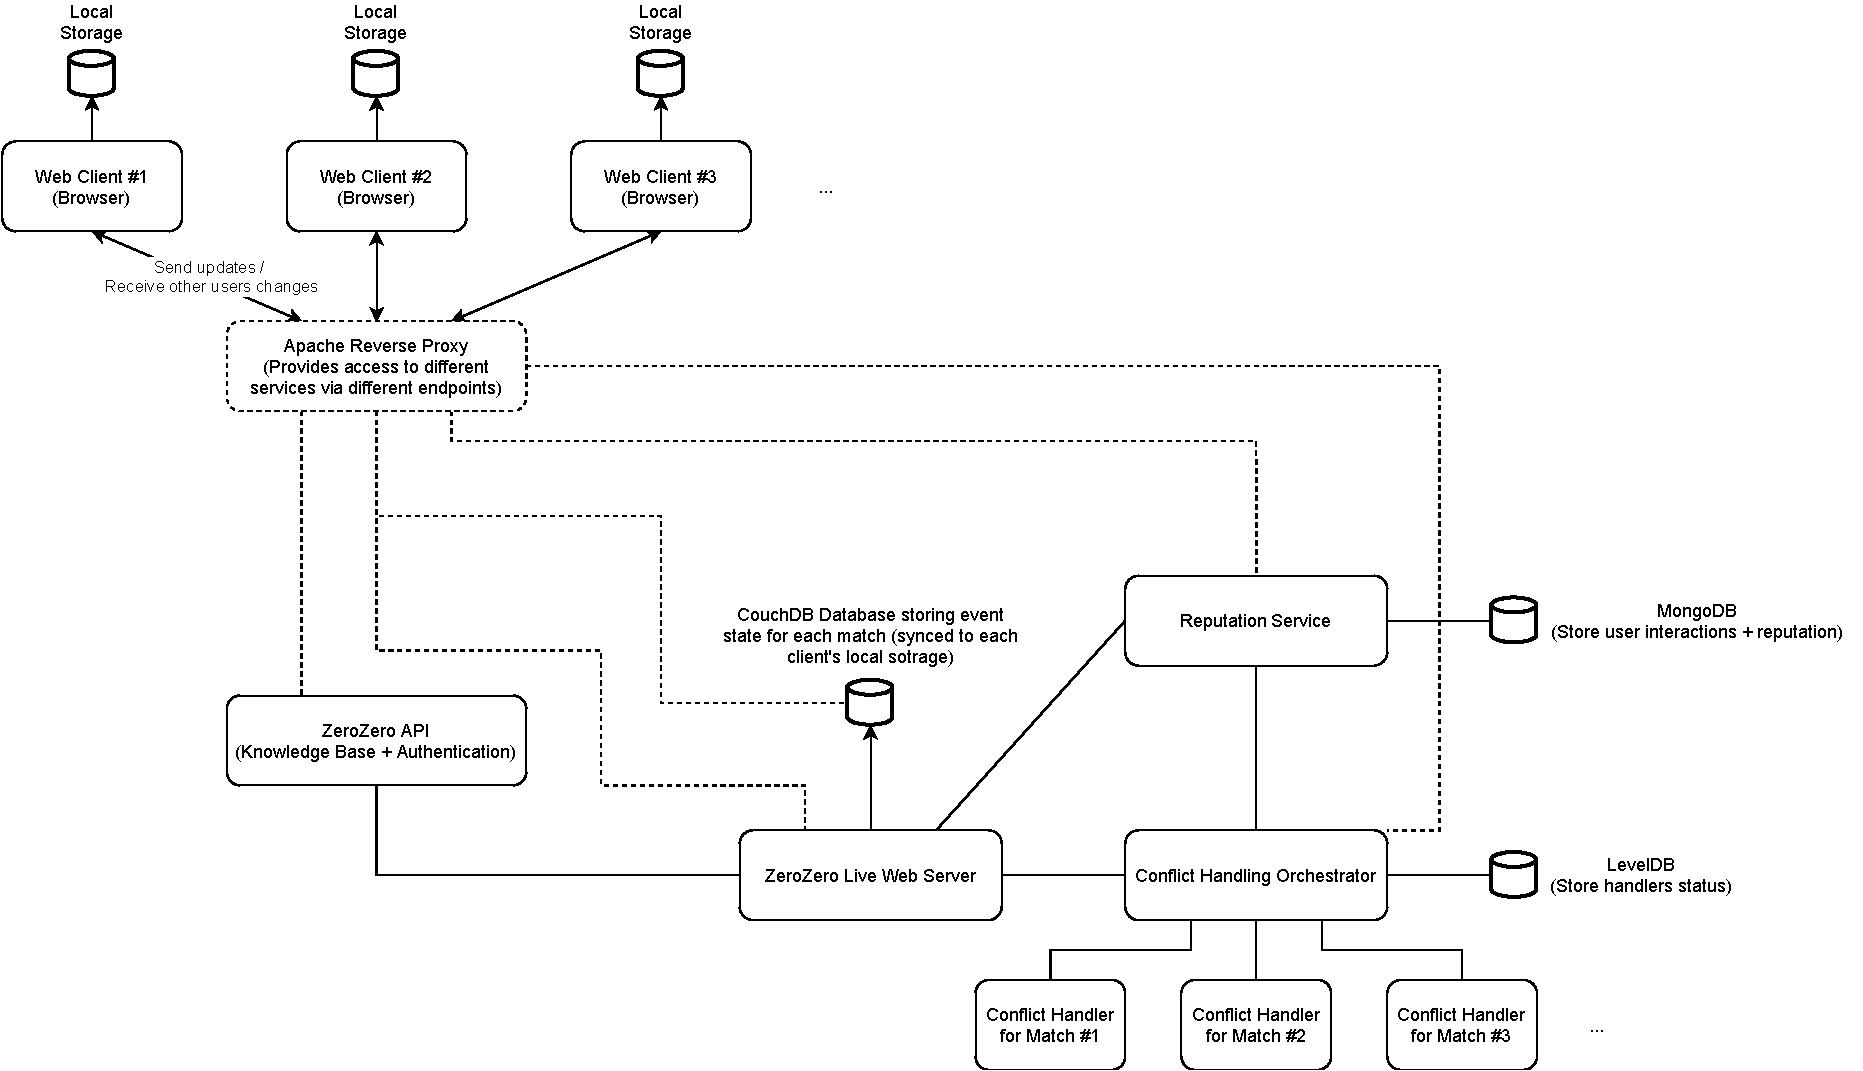
\includegraphics[width=0.5\textheight]{zerozerolive-arch.pdf}
%         % \caption{Services Architecture of the Application}
%     }

%     \end{figure}
    



%%----------------------------------------
%% Final materials
%%----------------------------------------

%% Bibliography
%% Comment the next command if BibTeX file not used
%% bibliography is in ``myrefs.bib''
\PrintBib{myrefs}

%% Index
%% Uncomment next command if index is required
%% don't forget to run ``makeindex pdis'' command
%\PrintIndex

\end{document}
